% This file was created by matplotlib2tikz v0.6.13.
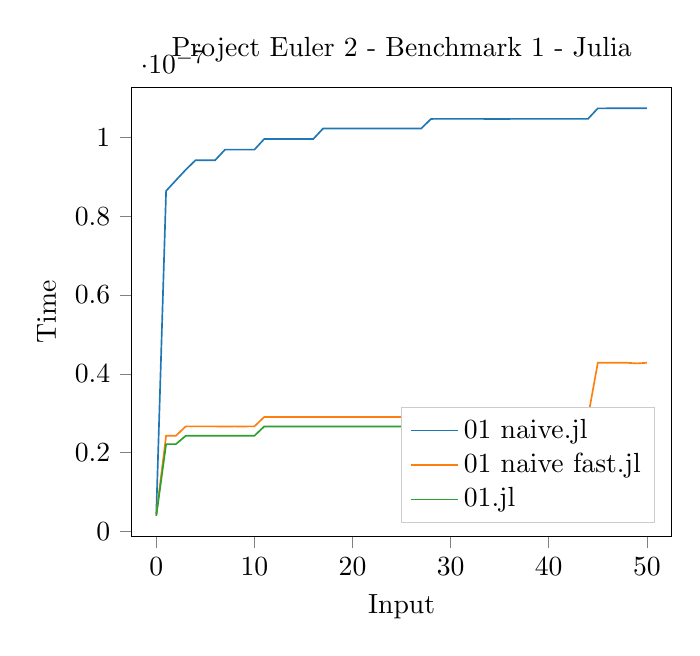
\begin{tikzpicture}

\definecolor{color1}{rgb}{1,0.498039215686275,0.0549019607843137}
\definecolor{color0}{rgb}{0.12156862745098,0.466666666666667,0.705882352941177}
\definecolor{color2}{rgb}{0.172549019607843,0.627450980392157,0.172549019607843}

\begin{axis}[
title={Project Euler 2 - Benchmark  1 - Julia},
xlabel={Input},
ylabel={Time},
xmin=-2.5, xmax=52.5,
ymin=-1.19880690550363e-09, ymax=1.12580945015576e-07,
tick align=outside,
tick pos=left,
x grid style={lightgray!92.026143790849673!black},
y grid style={lightgray!92.026143790849673!black},
legend style={at={(0.97,0.03)}, anchor=south east, draw=white!80.0!black},
legend entries={{01 naive.jl},{01 naive fast.jl},{01.jl}},
legend cell align={left}
]
\addlegendimage{no markers, color0}
\addlegendimage{no markers, color1}
\addlegendimage{no markers, color2}
\addplot [semithick, color0]
table {%
0 4.507e-09
1 8.64234693877551e-08
2 8.91257668711656e-08
3 9.17991803278689e-08
4 9.42299794661191e-08
5 9.42268993839836e-08
6 9.42268993839836e-08
7 9.68981481481481e-08
8 9.69002057613169e-08
9 9.690329218107e-08
10 9.69043209876543e-08
11 9.96e-08
12 9.95958762886598e-08
13 9.95927835051546e-08
14 9.96092783505155e-08
15 9.96010309278351e-08
16 9.95886597938144e-08
17 1.02277892561983e-07
18 1.02284090909091e-07
19 1.02288223140496e-07
20 1.0227479338843e-07
21 1.02285123966942e-07
22 1.02270661157025e-07
23 1.02276859504132e-07
24 1.0227479338843e-07
25 1.0228305785124e-07
26 1.02277892561983e-07
27 1.0227479338843e-07
28 1.04698757763975e-07
29 1.04714285714286e-07
30 1.04701863354037e-07
31 1.04707039337474e-07
32 1.04711180124224e-07
33 1.04708074534161e-07
34 1.04691511387164e-07
35 1.04690476190476e-07
36 1.0470082815735e-07
37 1.04712215320911e-07
38 1.04721532091097e-07
39 1.04707039337474e-07
40 1.04717391304348e-07
41 1.04709109730849e-07
42 1.04710144927536e-07
43 1.04718426501035e-07
44 1.04717391304348e-07
45 1.07386292834891e-07
46 1.07389408099688e-07
47 1.07398753894081e-07
48 1.07389408099688e-07
49 1.07409138110073e-07
50 1.07394600207684e-07
};
\addplot [semithick, color1]
table {%
0 4.239e-09
1 2.4285140562249e-08
2 2.42861445783133e-08
3 2.66653266331658e-08
4 2.66643216080402e-08
5 2.66653266331658e-08
6 2.66623115577889e-08
7 2.66603015075377e-08
8 2.66623115577889e-08
9 2.66582914572864e-08
10 2.66713567839196e-08
11 2.90502512562814e-08
12 2.90562814070352e-08
13 2.90482412060302e-08
14 2.90472361809045e-08
15 2.90462311557789e-08
16 2.90472361809045e-08
17 2.9046277665996e-08
18 2.90452261306533e-08
19 2.90492462311558e-08
20 2.90482412060302e-08
21 2.90472361809045e-08
22 2.90462311557789e-08
23 2.90573440643863e-08
24 2.90422535211268e-08
25 2.90462311557789e-08
26 2.90462311557789e-08
27 2.90472361809045e-08
28 2.90472361809045e-08
29 2.90492462311558e-08
30 2.90502512562814e-08
31 2.90462311557789e-08
32 2.9043216080402e-08
33 2.90482412060302e-08
34 2.9051256281407e-08
35 2.90492462311558e-08
36 2.90472361809045e-08
37 2.90492462311558e-08
38 2.90482412060302e-08
39 2.90472361809045e-08
40 2.90502512562814e-08
41 2.90532663316583e-08
42 2.90402010050251e-08
43 2.90482412060302e-08
44 2.9046277665996e-08
45 4.28128772635815e-08
46 4.28158953722334e-08
47 4.28058350100604e-08
48 4.2807847082495e-08
49 4.26599597585513e-08
50 4.28098591549296e-08
};
\addplot [semithick, color2]
table {%
0 3.973e-09
1 2.21646586345382e-08
2 2.21686746987952e-08
3 2.42761044176707e-08
4 2.4281124497992e-08
5 2.42751004016064e-08
6 2.42751004016064e-08
7 2.42751004016064e-08
8 2.42751004016064e-08
9 2.42781124497992e-08
10 2.4281124497992e-08
11 2.66552763819095e-08
12 2.6651256281407e-08
13 2.66552763819095e-08
14 2.66522613065327e-08
15 2.66522613065327e-08
16 2.66572864321608e-08
17 2.66542713567839e-08
18 2.66522613065327e-08
19 2.66522613065327e-08
20 2.66532663316583e-08
21 2.66552763819095e-08
22 2.66542713567839e-08
23 2.66542713567839e-08
24 2.66562814070352e-08
25 2.66542713567839e-08
26 2.66562814070352e-08
27 2.66562814070352e-08
28 2.66582914572864e-08
29 2.66552763819095e-08
30 2.66613065326633e-08
31 2.66542713567839e-08
32 2.66532663316583e-08
33 2.66542713567839e-08
34 2.66542713567839e-08
35 2.66613065326633e-08
36 2.66542713567839e-08
37 2.66542713567839e-08
38 2.66562814070352e-08
39 2.66592964824121e-08
40 2.66562814070352e-08
41 2.66582914572864e-08
42 2.66522613065327e-08
43 2.66522613065327e-08
44 2.66532663316583e-08
45 2.87678391959799e-08
46 2.87698492462312e-08
47 2.87708542713568e-08
48 2.87688442211055e-08
49 2.87698492462312e-08
50 2.87718592964824e-08
};
\end{axis}

\end{tikzpicture}